%%%%%%%%%%%%%%%%%%%%%%%%%%%%%%%%%%%%%%%%%
% Simple Sectioned Essay Template
% LaTeX Template
%
% This template has been downloaded from:
% http://www.latextemplates.com
%
% Note:
% The %\lipsum[#] commands throughout this template generate dummy text
% to fill the template out. These commands should all be removed when 
% writing essay content.
%
%%%%%%%%%%%%%%%%%%%%%%%%%%%%%%%%%%%%%%%%%

%----------------------------------------------------------------------------------------
%	PACKAGES AND OTHER DOCUMENT CONFIGURATIONS
%----------------------------------------------------------------------------------------

\documentclass[12pt]{article} % Default font size is 12pt, it can be changed here

\usepackage[spanish]{babel}%Para el español
\usepackage[utf8]{inputenc}%para los acentos
\usepackage{amsmath,amssymb,amsfonts,amsthm}
\usepackage{graphicx}
\usepackage{bbm}
\usepackage{textcomp}
\usepackage{amstext}

\usepackage{geometry} % Required to change the page size to A4
\geometry{a4paper} % Set the page size to be A4 as opposed to the default US Letter

\usepackage{graphicx} % Required for including pictures

\usepackage{float} % Allows putting an [H] in \begin{figure} to specify the exact location of the figure
\usepackage{wrapfig} % Allows in-line images such as the example fish picture

\linespread{1.2} % Line spacing

%\setlength\parindent{0pt} % Uncomment to remove all indentation from paragraphs

\graphicspath{{Imagenes/}} % Specifies the directory where pictures are stored

\usepackage{tikz}
%%%<
%\usepackage[spanish]{babel}%Para el español
%\usepackage[utf8]{inputenc}
%\usepackage{verbatim}
\usepackage{listings}
\usepackage{xcolor}
\usepackage{textcomp}
%\usepackage{times}

\usetikzlibrary{shadows}
\usetikzlibrary{shapes.symbols}

\def\codefont{
%\fontspec{Courier New}
\fontsize{9pt}{11pt}\selectfont}
\definecolor{codebgcolor}{HTML}{EDEDED}
\newenvironment{code}
{\begin{center}
\begin{tikzpicture}
\node [shade,%rellena el fondo con un gradiente
	   top color=black!1,%parametro de gradiente
	   bottom color=black!12,%parametro de gradiente
	   %draw,%dibuja la línea de contorno 
	   drop shadow,%dibuja una sombra
	   %fill=codebgcolor,%rellena el fondo con color plano
	   rounded corners=5pt,	   
	   ]
\bgroup
\bgroup\codefont
\begin{tabular}{l}}
{\end{tabular}
\egroup
\egroup;
\end{tikzpicture}
\end{center}}
 
\definecolor{dkgreen}{rgb}{0,0.6,0}

\lstset{
	language=C,
	literate=%
	{á}{{\'{a}}}1
	{é}{{\'{e}}}1
	{í}{{\'{i}}}1
	{ó}{{\'{o}}}1
	{ú}{{\'{u}}}1
	{ñ}{{\~{n}}}1
	{<}{{$<$}}1
	{>}{{$>$}}1,
	basicstyle=\footnotesize\ttfamily,
	keywordstyle=\bfseries, 
	comment=[l]{\;},%
	breaklines=true,
	prebreak = \raisebox{0ex}[0ex][0ex]{\ensuremath{\hookleftarrow}},
    }

\usepackage{framed}

\begin{document}


%----------------------------------------------------------------------------------------
%	TITLE PAGE
%----------------------------------------------------------------------------------------

\begin{titlepage}
\newgeometry{left=1.5cm,right=1.5cm}

\newcommand{\HRule}{\rule{\linewidth}{0.5mm}} % Defines a new command for the horizontal lines, change thickness here

\center % Center everything on the page

\textsc{\LARGE Universidad Nacional de Córdoba}\\[1.5cm] % Name of your university/college
\textsc{\Large Informe Trabajo Final}\\[0.5cm] % Major heading such as course name
\textsc{\large Algoritmos y Estructuras de Datos}\\[0.5cm] % Minor heading such as course title

\HRule \\[0.4cm]
{ \huge \bfseries Aplicación del algoritmo de Dijkstra para la simulación del trafico de paquetes en una red de routers y computadoras}\\[0.4cm] % Title of your document
\HRule \\[1.5cm]

\begin{minipage}{0.4\textwidth}
\begin{flushleft} \large
\emph{Autores:}\\
Esteban \textsc{Morales} (35.104.714)\\
Adelina \textsc{Mayol} (34.140.737)\\
Guillermo \textsc{Valetti} (35.177.596)\\
\end{flushleft}
\end{minipage}
~
\begin{minipage}{0.4\textwidth}
\begin{flushright} \large
\emph{Supervisores:} \\
Gustavo \textsc{Wolfmann}\\ % Supervisor's Name
Rubén \textsc{Ayme}
\end{flushright}
\end{minipage}\\[4cm]

{\large \today}\\[3cm] % Date, change the \today to a set date if you want to be precise

%\includegraphics{Logo}\\[1cm] % Include a department/university logo - this will require the graphicx package

\vfill % Fill the rest of the page with whitespace
\restoregeometry
\end{titlepage}

%----------------------------------------------------------------------------------------
%	TABLE OF CONTENTS
%----------------------------------------------------------------------------------------

\tableofcontents % Include a table of contents

\newpage % Begins the essay on a new page instead of on the same page as the table of contents 

%----------------------------------------------------------------------------------------
%	INTRODUCTION
%----------------------------------------------------------------------------------------

\section{Introducción} % Major section

El siguiente informa, expone el desarrollo del Trabajo final de la materia Algorítmos y Estructuras de datos.

La consigna demanda la implementación  del algoritmo de Dijkstra  o  “del menor camino” a la simulación del trafico de  paquetes por una Red de Routers y computadoras, conectados entre si, que responden a una configuración inicial.

El objetivo principal, es obtener  el camino mas corto para el recorrido de los paquetes a través de la red mediante el algoritmo de Dijkstra, y asi poder valuar las tablas de cada uno de los routers, para que puedan redirigir los paquetes con destino a routers vecinos, o bien, armar la pagina si el destino es el propio router.

%------------------------------------------------

\section{Desarrollo} % Sub-section
El desarrollo tiene una primera fase donde se interpreta la consigna, para conocer el sistema (red de routers) a simular. Se realizo una descripción e implementación con orientación a objeto, permitiendo modularidad y hacer uso de herencia entre las clases Arco – Conexión.
Para ello, fueron necesarios los conocimientos brindados en clase de las estructuras implementadas como Nodo, Lista, Cola, Colas Anidadas, Grafo.
Una vez proyectado el sistema, en la segunda fase con la codificamos y adaptamos del  Algoritmo de Dijkstra al sistema, dado que el resultado devuelto por el algoritmo, no es un valor de uso directo.
Por consigna, sabemos que los routers no son dispositivos autodidactas, es por ello, que existe un  ’Administrador’ que  cumple la función de gestionar, entre otras cosas,  la ejecución del algoritmo al inicio y cada 30 ciclos, que restablece los valores de las tablas de redireccionamiento de paquetes de cada Router perteneciente a la red. Es por ello, que a  partir del cálculo hecho por  el algoritmo, paralelamente se trazan las trayectorias más eficientes, es decir, la  secuencia de routers más eficiente.
La tercera fase, para verificar el modelo, realizamos 3 casos de uso, corroborando los valores arrojados por el algoritmo, y las tablas calculadas para cada router.

\section{Primera Fase: Diseño e Implementación del Sistema} % Sub-section

\subsection{Consigna}

Desarrollar un programa que simule el trafico de datos, al \"estilo\" del funcionamiento de Internet.

Existen (n) maquinas que cumplen la función de routers: enrutan los datos desde la maquina de origen hacia la maquina de destino.

Existen otras (k) maquinas que son las emisoras - receptoras de paginas. Cada una de estas maquinas esta conectada a un único router que es el encargado de enviar/recibir las paginas hacia/desde el destino final.

Cada router esta conectado a 1 o mas routers. Cada router sabe cuales son las maquinas finales a las cuales esta conectado y cuales son los routers vecinos que tiene, es decir a que otros routers esta conectado directamente.

Ademas cada router tiene una tabla que le indica a que router enviar los datos con un determinado destino.

Cada router tiene una conexión directa con sus vecinos de un determinado ancho de banda.

Cuando un router recibe de una de sus maquinas terminales una página para enviar, este lo divide en n paquetes de igual tamaño y va enviando por la ruta elegida de a un paquete por vez. Es decir que un servicio pedido por una maquina cliente se divide y se envía de a tramos.

A su vez, cuando un router va recibiendo de otro router paquetes con un determinado destino, debe reenviarlo al router correspondiente en la ruta, o bien, si el destino final es una maquina a la cual esta conectado directamente, debe ir almacenando los paquetes recibidos hasta que estén todos los que correspondan a la pagina enviada, rearma la pagina y recién allí se la envía a la maquina destino.

Las direcciones de las maquinas, son tipo IP, pero simplificadas. Tienen dos partes de 1 byte cada una: la primera indica el router y la segunda la maquina conectada al router. Es decir que pueden haber 256 routers con 256 maquinas cada uno.

Como hace cada router para computar la tabla de destinos que posee?

Si la dirección del paquete corresponde a la de un router vecino, hay una conexión directa, por lo que no hay mas tramite. Para routers que no son vecinos pueden haber varias rutas alternativas, debiendo el router elegir aquella que tiene la menor carga de trafico. Una vez determinada la mejor ruta, todos los paquetes enviados a un determinado destino, se envían al router vecino que conforma el camino elegido.

En resumen, cada router tiene las siguientes funciones:

a) recibir una pagina de una maquina cliente, dividirla en los paquetes que corresponda, y enviarla a la cola de trafico de la ruta que corresponda

b) recibir paquetes de los routers vecinos y redireccionarlos hacia el router que corresponda si la dirección del paquete no es la propia del router, o bien si la dirección del paquete es la del router en cuestión, debe esperar a recibir todos los paquetes que corresponden a la pagina enviada y una vez sucedido esto, enviar la pagina a la maquina de destino.

Cada router tiene una cola de envíos para cada router vecino, en donde van encolando los paquetes que tienen que enviarse por ese canal y envía por cada ciclo, todos los que su ancho de banda le permita. En la cola no se deben colocar todos los paquetes de una pagina consecutivos: deben ser intercalados con los paquetes que provengan de otra maquina, para que se vayan enviado parcialmente de todas las maquinas al mismo tiempo. Esto evita que un envió muy pesado atore al server y los otros paquetes demoren mucho en ser enviados.

Existe un administrador del sistema que de vez en cuando recomputa las rutas optimas de todos los routers. Para ello cada router le envía el tamaño de la cola de espera de envíos de paquetes hacia cada router vecino, y con ello el administrador determina la ruta optima pasando por los routers que tengan menor trafico pendiente. Hay que tener en cuenta que cada router envía (k) paquetes por vez en un canal, según el ancho de banda que tenga el canal.

Para determinar el optimo, lo que importa es la cantidad de ciclos que un nuevo paquete debe esperar hasta ser enviado. Ademas se pierde un ciclo al entrar a un router y volver a salir.

O sea que si un router tiene la cola vacía, no tiene un costo de cero, si no de uno, porque el paquete debe esperar hasta el próximo ciclo para ser reenviado.

Una vez que el administrador determina los caminos óptimos, se los informa a cada router.

Esos caminos son utilizados a partir de ese momento hasta que vuelven a recomputarse.

Puede pasar que los paquetes pendientes de enviar de una pagina, utilicen un camino distinto de los enviados previamente, porque se cambio el camino a utilizar por uno con menos trafico.

El caso es el así: la pagina se dividió en 50 paquetes. Se enviaron 20. Se recomputa el camino optimo y se cambia de ruta. Los 30 paquetes restantes van por otra ruta, que al ser tomada como optima, se pueden llegar a destino antes que los primeros 20. Tener esto en cuenta cuando el router debe rearmar la pagina.

Usted deberá simular todo esto. Para ello construirá un ciclo donde se le dará turno a todos los routers para que hagan las tareas que tienen que hacer por vez. Cada 30 ciclos, tomara el control el administrador para recomputar los caminos óptimos y volverán a computarse los ciclos.

Deberá utilizar números aleatorios para simular la generación de paginas a ser enviadas, el destino y el tamaño de cada pagina.

La cantidad de routers, la cantidad de terminales por router, las conexiones directas de los routers y el ancho de banda entre los routers y entre cada terminal y el router asociado deberá ser configurable y definido en un archivo que se utilizara para parametrizar el sistema.

Dada la magnitud del trabajo, aconsejo, diciendo esto con un tono de casi imposición, trabajar en equipos de 2 o 3 personas para dividirse el trabajo. También aconsejo tomarse al menos una semana para pensar como armar el sistema, haciendo un análisis detallado en profundidad de los requerimientos y de la implementación de la solución, antes de programar una sola linea de código.
%------------------------------------------------
\subsection{Diagrama de Clases}

\subsection{Primera versión}
De la interpretación de la consigna se realizó un análisis sistemico del problema, obtuvimos un perspectiva general del sistema, sus componentes y la interfaz necesaria, el resultado es representado a partir del siguiente diagrama de clases en su primera forma.

\begin{figure}[H] % Example image
\center{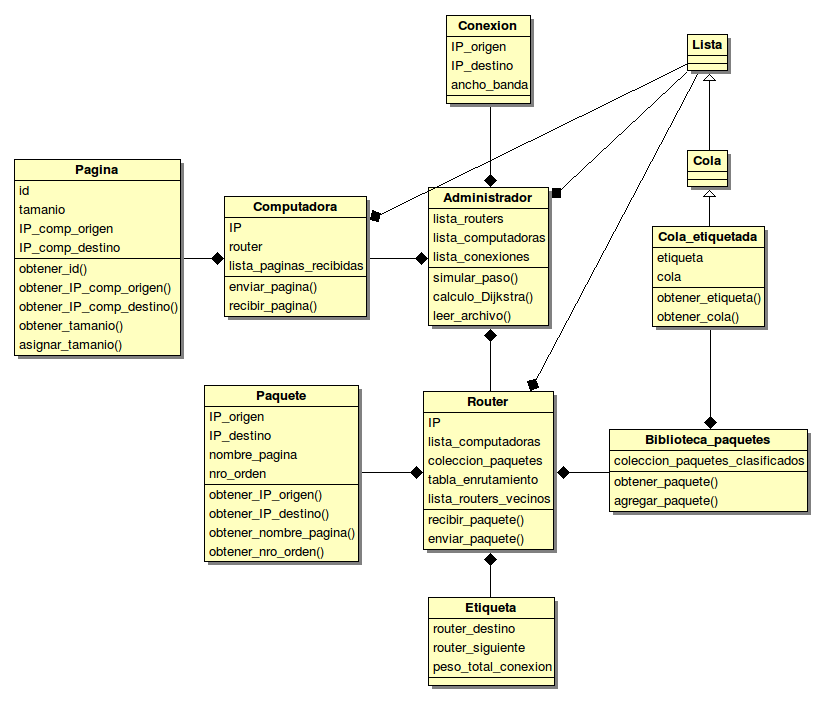
\includegraphics[width=\linewidth]{DiagramaClases_v1}}
\caption{Primer Diagrama de Clases.}
\label{fig:speciation}
\end{figure}

\subsection{Segunda Versión}
De la implementación surgieron modificaciones del modelo inicial, en la segunda versión se determinaron todas las clases a usar en el diseño.

\begin{figure}[H] % Example image
\center{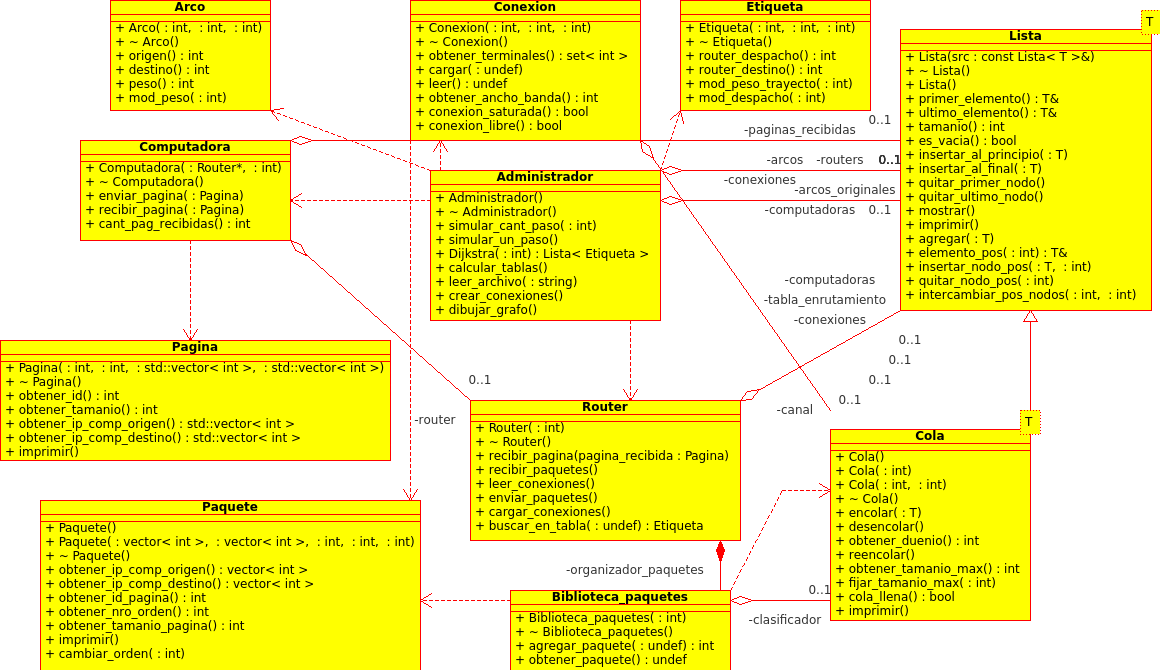
\includegraphics[width=\linewidth]{Diagrama_Clases_Final_AyED}}
\caption{Segunda versión del diagrama de clases.}
\label{fig:DC_v2}
\end{figure}

\subsection{Versión Final}
Luego de muchos cambios (Todos comentados en el repositorio de github) sobre las clases, esto es inclusión, remosión y modificación de campos y métodos, se obtuvo el diagrama final.

\begin{figure}[H] % Example image
\center{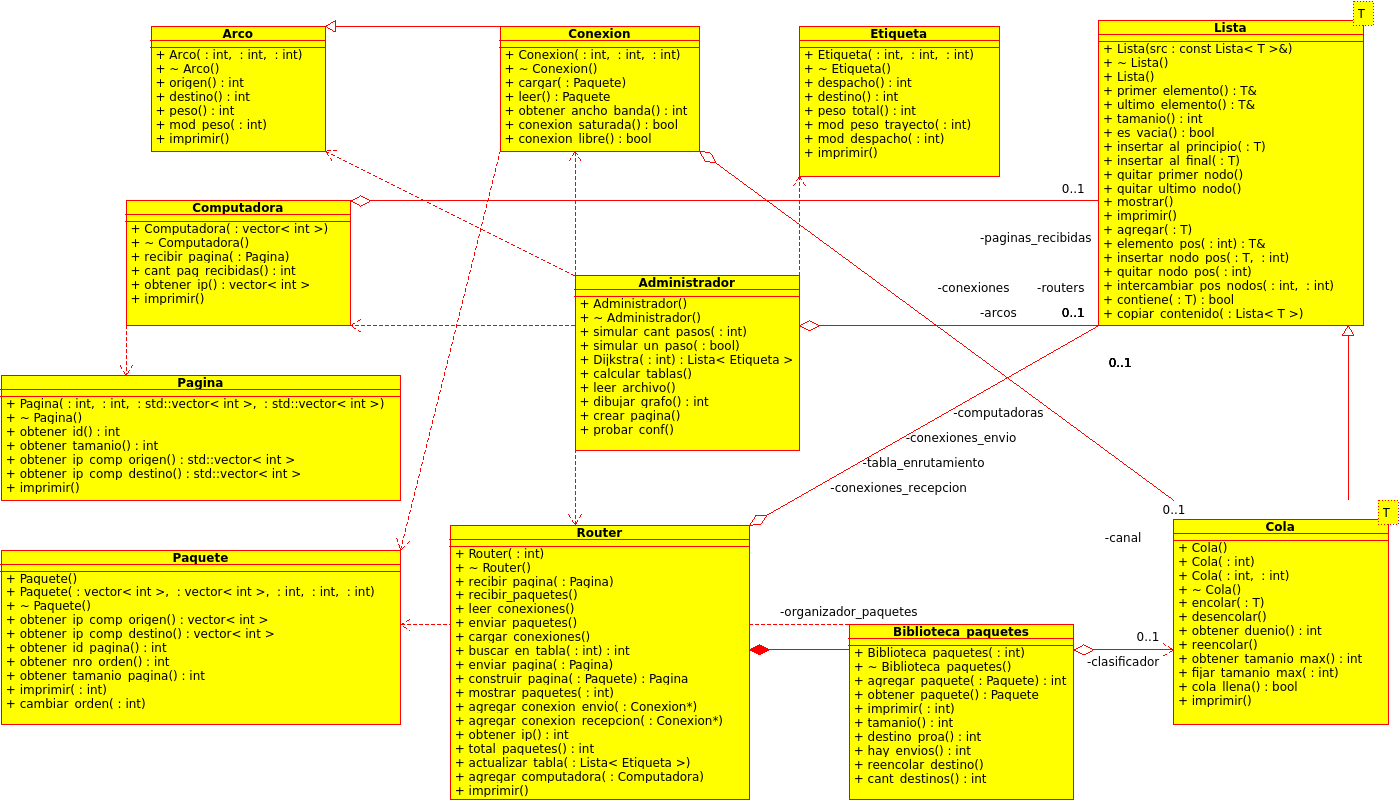
\includegraphics[width=\linewidth]{Diagrama_Clases_Final_AyED_v2}}
\caption{Diagrama de clases final.}
\label{fig:DC_vF}
\end{figure}

\section{Clases}
\subsection{Estructuras}
Las estructuras de datos son los objetos que permiten la organización de los datos, colecciones de objetos o referencias de manera que puedan administrarse eficientemente.
En el caso del presente trabajo se utilizaron 2 estructuras, a saber:
\begin{itemize}
\item Lista
\item Cola
Como son estructuras de funcionamiento ampliamente documentado se omite la explicación.
\end{itemize}
\subsection{Objetos}
Con el objetivo de modularizar el código y procurar el encapsulamiento de cada parte, mediante la interpretación sistemática de la consigna se decidió la implementación de las siguientes clases:
\begin{itemize}
\item Administrador
\item Arco
\item Biblioteca\_paquetes
\item Computadora
\item Conexion
\item Etiqueta
\item Pagina
\item Paquete
\item Router
\end{itemize}
A continuación se describe cada una de ellas y se detallan los métodos más relevantes.
\subsubsection{Administrador}
Esta clase se encarga de administrar la simulación. Puede ver y modificar absolutamente todos los parámetros de la red Routers, computadoras, conexiones. Tiene la funcionalidad de calcular caminos óptimos con la implementación del algoritmo de Dijkstra para grafos direccionados y que admite ciclos no recurrentes. Adicionalmente es capáz de leer la configuración de la red desde un archivo y dibujar el grafo de la red haciendo uso de la librería graphvz mediante la aplicación dot de los repositorios de ubuntu.
Cabe mensionar que se determinó que todos routers tienen la misma cantidad de maquinas conectadas.
\subsubsection{Arco}
Esta clase representa el arco o la arista de un grafo. Es la entidad que conecta dos nodos o vértices y que se le asigna un peso o distancia.
\subsubsection{Biblioteca\_paquetes}
Esta clase es la estructura de datos que garantiza justicia en el envío de paquetes, esto es, igual atención a las solicitudes de todos los routers y para todas las páginas. En su interiror se implementa una colección de tipo anidada de tres niveles que se usa para organizar los paquetes. Esta colección es del tipo cola y utiliza el campo especial duenio para identificar a qué router y página pertenecen los paquetes encolados.
\subsubsection{Computadora}
Esta clase representa las computadoras o terminales conectadas a los routers en la red a simular. Incluye un puntero al router al que está conectada con el objetivo de solicitarle el envío de una nueva página. Adicionalmente posee una lista de páginas recibidas que podrá ser usada para medir la eficiencia de la red.
\subsubsection{Conexion}
Esta clase representa la vía que comunica dos routers en la red y hace referencia al arco del grafo de la red a simular. Consta de dos nros de ip, el origen y destino así como la especificación del ancho de banda y una cola para emular las limitaciones del canal. 
\subsubsection{Etiqueta}
Esta clase implementa las triplas de tres enteros que utilizará la clase router para determinar hacia dónde debe enviar los paquetes.
\subsubsection{Pagina}
Esta clase representa las páginas que generan las computadoras y que contiene una identificación su tamaño en cantidad de paquetes y las direcciones de origen y de destino en forma de duplas de enteros.
\subsubsection{Paquete}
Esta clase representa las que componen una página y que contiene un número de órden, el tamanio de la página a la que pertenece y las direcciones de origen y de destino en forma de duplas de enteros.
\subsubsection{Router}
Esta clase representa los nodos de la red y opera como enrutador, tiene las funcionalidades de enviar y recibir paquetes así como recibi páginas completas desde las computadoras que están conectadas a este router. La recepción del paquete se realiza mediante la lectura de sus conexiones de recepción y el envío mediante la carga de las conexiones de envío. Cada router tiene una identificación entera, una colección de computadoras, una lista de conexiones de envío y otra de recepción, además cuenta con una tabla de enrutamiento que contiene las etiquetas para cada destino.
%------------------------------------------------

\section{Segunda Fase: Implementación del Algoritmo} % Sub-sub-section
\textit{Algoritmo Implementado: Dijkstra}\\
El algoritmo de Dijkstra resuelve el problema de los caminos más cortos y orígen único en un  grafo dirigido y ponderado $G=(V,E)$ tal que todos los pesos de los arcos son no negativos. Con una buena implementación el timepo de ejecución del algoritmo de Dijkstra es menor al de Bellman-Ford.

\textit{¿Para qué sirve el algoritmo?}\\
La función del algoritmo es calcular los caminos mínimos que hay entre el nodo origen y todos los nodos del grafo.
\textit{¿Cuál es  la lógica del algoritmo?}\\
 El algoritmo parte de un nodo inicial, y se va desplazando a través de  la red, guiándose por los nodos adyacentes al nodo actual. 
Conforme el algoritmo evoluciona se encuentran mejores caminos para determinado nodo destino por lo que se actualiza el resultado. Finalmente el algoritmo termina cuando no quedan nodos sin camino mínimo encontrado.

Dijkstra mantiene un conjunto $S$ de nodos para los que ya se calcularon los caminos mínimos. El algoritmo cíclicamente selecciona un nodo $u \in (V-S)$ cuya distancia es la mínima entre los que quedan sin procesar, agrega el nodo seleccionado $u$ a $S$ y \textsc{ Relaja} todos los vértices adyacentes a $u$.

\begin{leftbar}
\textsc{Dijkstra}(G, nodo\_inicio)\\
1\indent	\textsc{Inicializar}(G)\\
2\indent	$S=\emptyset$\\
3\indent	$Q=G.V$\\
4\indent	\textbf{while} ($Q\neq\emptyset$)\\
5\indent\indent		nodo\_sel=\textsc{Mas Cercano}(Q)\\
6\indent\indent		$S=S\cup nodo\_sel$\\
7\indent\indent		\textbf{for each} $nodo\_i \in G.Adyacentes[nodo\_sel]$\\
8\indent\indent\indent			\textsc{Relajar}(u,v) 
\end{leftbar}

¿Como fue implementada dicha lógica?  Los elementos  que utilizamos son:
\begin{itemize}
\item Conjunto Q: conjunto de nodos no chequeados
\item Conjunto S: conjunto de nodos chequeados
\item Conjunto Adyacentes: conjunto de nodos adyacentes al nodo inicio
\item Vector Predecesores: guarda los valores de los router predecesores a cada router
\item Vector Distancias: almacena las distancias de los caminos mas cortos a cada router
\item Lista de Etiquetas: contiene las etiquetas correspondiente a cada uno de los routers, con los valores en el siguiente formato \\
\verb+{ r_destino, r_siguiente, peso del trayecto }+
\end{itemize}

Primeramente, cargamos en conjunto Q , Adyacentes, las etiquetas, haciendo distinción para la etiqueta del nodo inicio \verb+{ orden_nodo_inicio, 0,0 }+ y las demás \verb+{ orden_nodo_x, -1, INF }+.
Luego recorremos en conjunto Q buscando en las etiquetas de cada uno de los routers, la que contenga el menor trayecto. Con esta condición, seleccionamos el nodo actual o elegido, y lo pasamos al conjunto S.
Luego recorremos los arcos, buscando aquellos que tengan origen en el nodo actual, y que su destino no corresponda a un nodo contenido en S. 
Es entonces, cuando realizamos la comparación de distancias (trayectos almacenados en las etiquetas), con la distancia resultante de la suma de la distancia del trayecto desde el nodo inicio, al nodo actual, las la del trayecto del nodo actual al siguiente para determinar si actualizar o no los valores tanto en el peso de trayectoria, perteneciente a la etiqueta del router siguiente,  como en el Vector Distancias y Predecesores.

Seguidamente, normalizo y actualizo los valores en el Vector Predecesor, con los correspondientes valores de nodos adyacentes al nodo inicio, lo que nos permite posteriormente, armar las tablas para dicho router.
Finalmente, Se actualiza el campo \verb+r_siguiente+ de la etiqueta con el valor correspondiente,  calculado en dicho Vector de Predecesores. Terminando así la ejecución del algoritmo, devolviendo la tabla con los nuevos valores de redireccionamiento.
 
¿Qué diferencia tiene con Floyd-Warshall? Ambos algoritmos tienen la misma finalidad, obtener el calculo del camino mas corto. Pero la diferencia es que Dijkstra calcula los caminos partiendo desde un único nodo base, hasta los demás del grafo, mientras Floyd aplica lo mismo, pero para todos los nodos de la red.
Es decir, si el costo de calculo de Dijkstra es $n \times n$  operaciones, el costo de FFloyd-Warshall será $n \times n \times n$
%------------------------------------------------
\section{Tercera Fase: Pruebas}
Para la validacion del modelo, se realizaron corridas del programa para dos configuraciones con 5,  y 10 routers.
Realizamos capturas de pantallas de (a)Red y (b)Configuración inicial de Arcos para evidenciar la correcta recepción de información a partir del archivo de texto leído.

También capturamos los resultados arrojados por el algoritmo:
(c)en cuanto a distancias $\rightarrow$ (c)Vector Distancia
(d)respecto al router siguiente a direccionar $\rightarrow$ (d)Vector Predecesores
(e)el resultado final para cada router $\rightarrow$ (e)Tablas.

Finalmente, se realiza el seguimiento visual de los paquetes de la página (en amarillo), a lo largo de las conexiones de la red hasta que llega a Destino.

Caso 1: Red de 10 Routers, se realiza el seguimiento de la Pagina 5, de tamaño 5, que se dirige desde el Router 7 al Router 4.

\begin{figure}[H] % Example image
\center{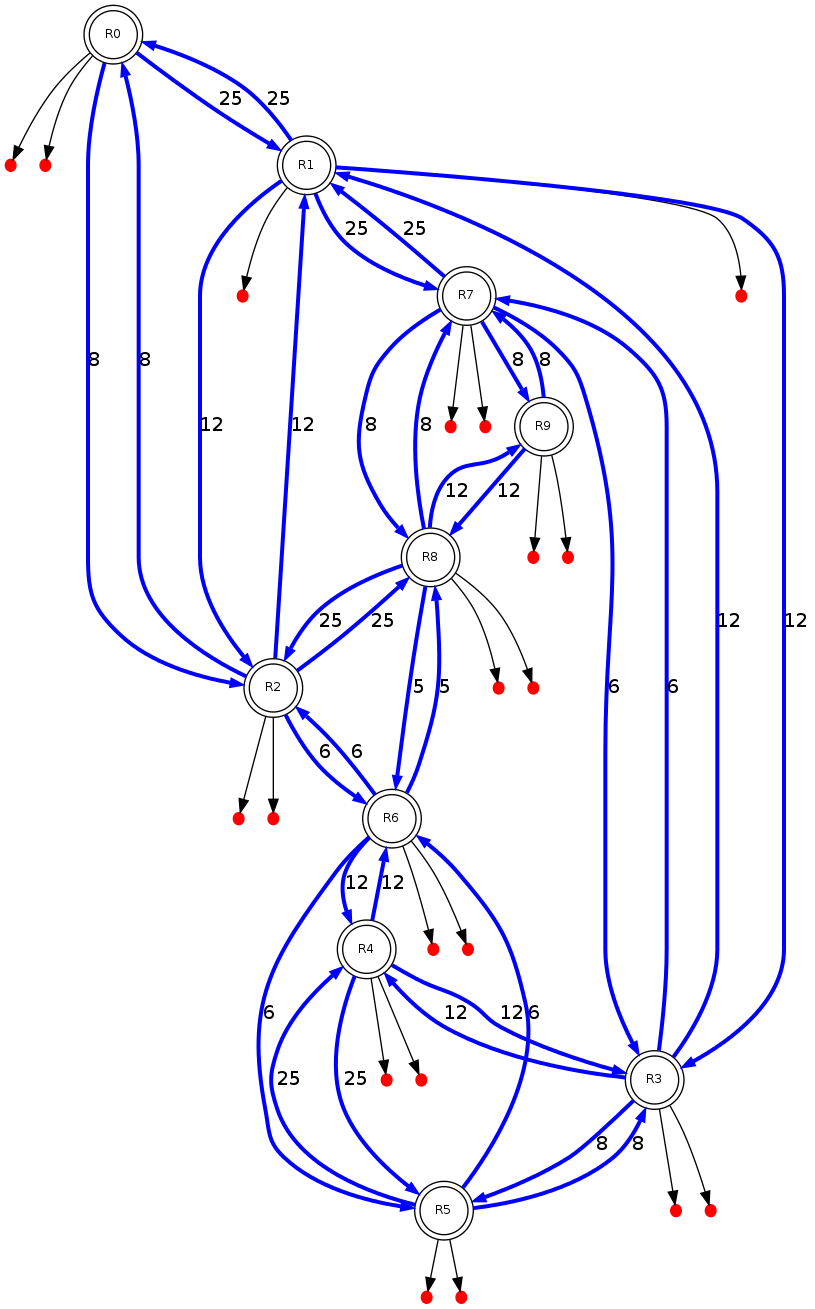
\includegraphics[width=\linewidth]{config_1_A}}
\label{fig:config_1_A}
\end{figure}

\begin{figure}[H] % Example image
\center{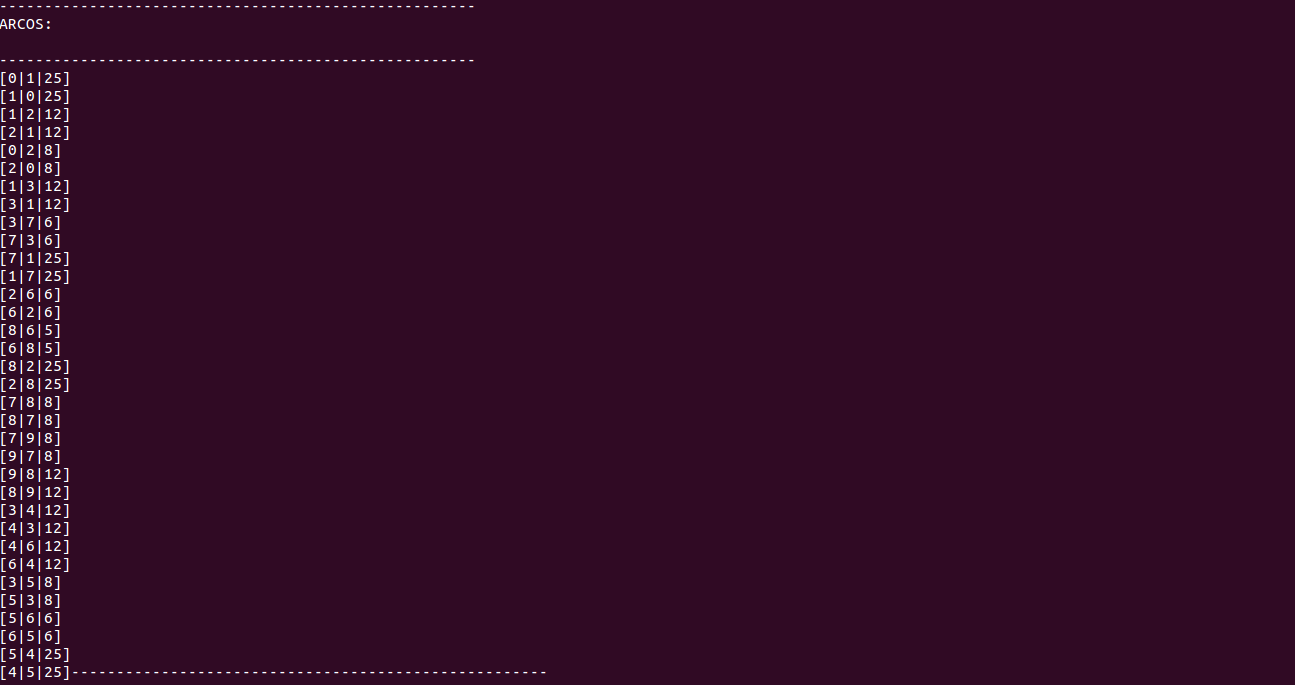
\includegraphics[width=\linewidth]{config_1_B}}
\label{fig:config_1_B}
\end{figure}

La trayectoria del paquete, según dijkstra, será a través de los siguientes routers: 7 $\rightarrow$ 3 $\rightarrow$ 4 con un peso de 18. Lo podemos ver en las tablas calculadas del direccionamiento

\begin{figure}[H] % Example image
\center{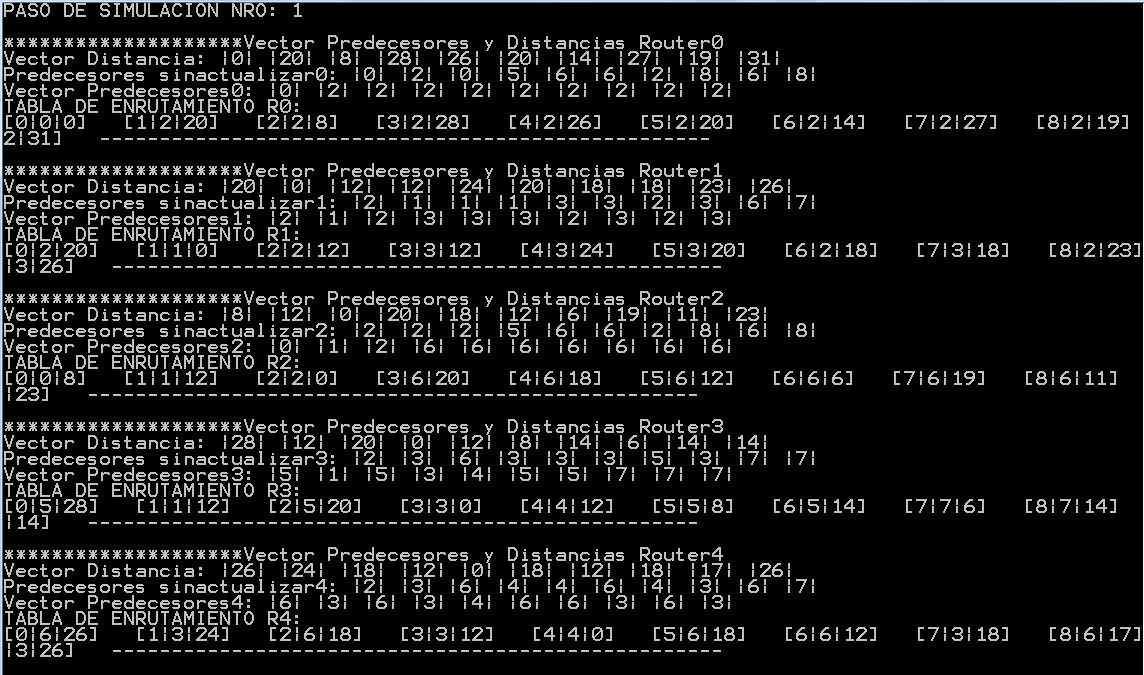
\includegraphics[width=\linewidth]{config1_C_D_y_E}}
\label{fig:config_1_C_D_y_E}
\end{figure}

\begin{figure}[H] % Example image
\center{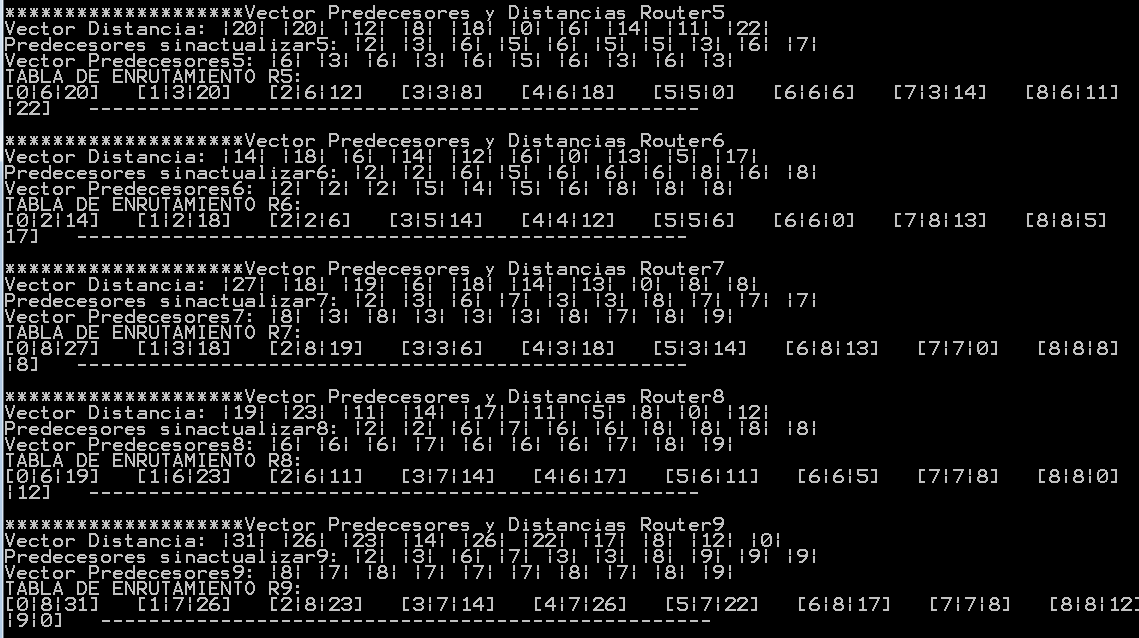
\includegraphics[width=\linewidth]{config1_C_D_y_E_2}}
\label{fig:config_1_C_D_y_E_2}
\end{figure}

Comenzamos el seguimiento de los paquetes de color amarillo.

\begin{figure}[H] % Example image
\center{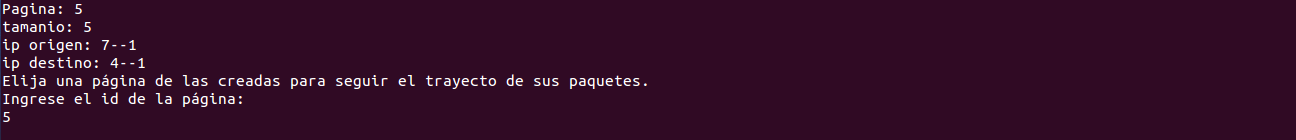
\includegraphics[width=\linewidth]{config_1_run1}}
\label{fig:config_1_run1}
\end{figure}

\begin{figure}[H] % Example image
\center{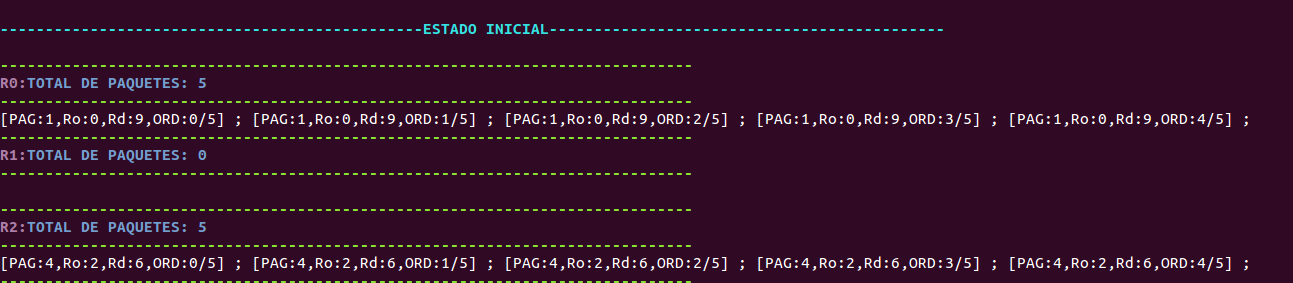
\includegraphics[width=\linewidth]{config_1_run2}}
\label{fig:config_1_run2}
\end{figure}

\begin{figure}[H] % Example image
\center{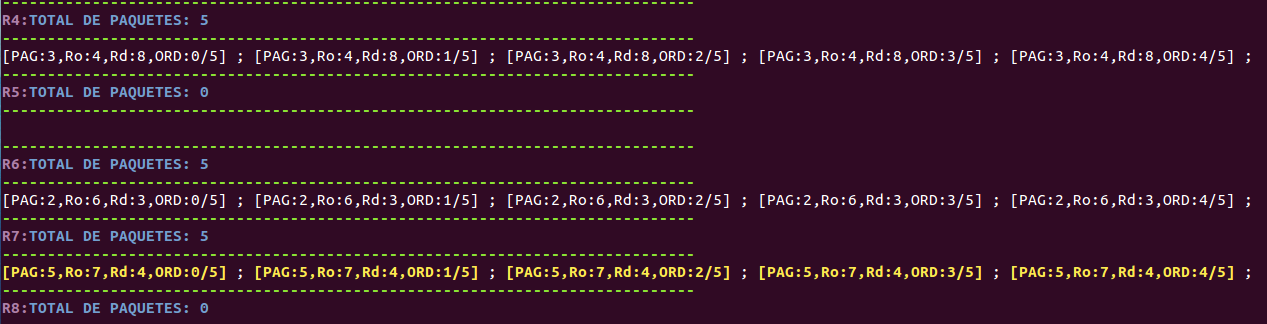
\includegraphics[width=\linewidth]{config_1_run3}}
\label{fig:config_1_run3}
\end{figure}

\begin{figure}[H] % Example image
\center{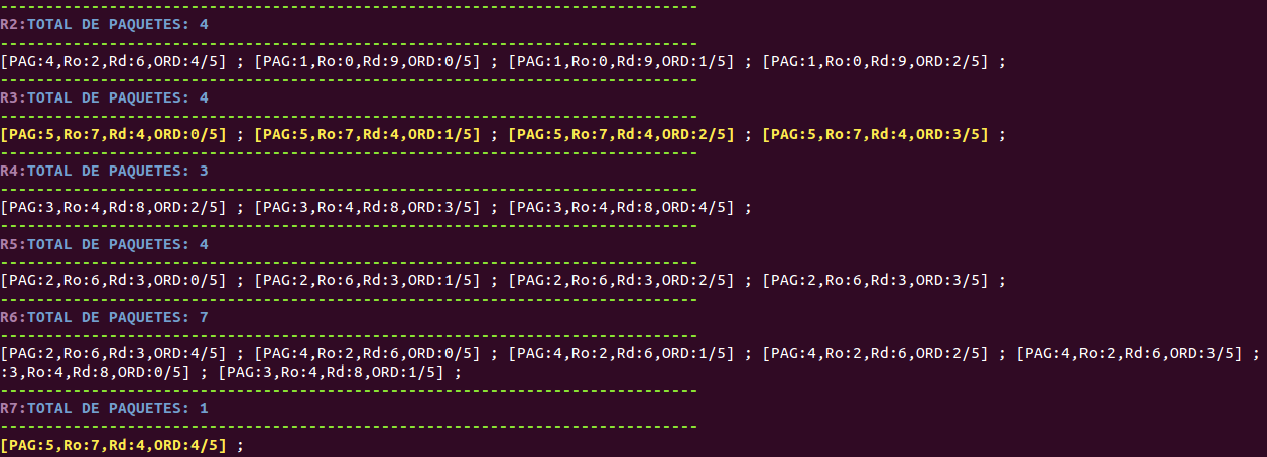
\includegraphics[width=\linewidth]{config_1_run4}}
\label{fig:config_1_run4}
\end{figure}

\begin{figure}[H] % Example image
\center{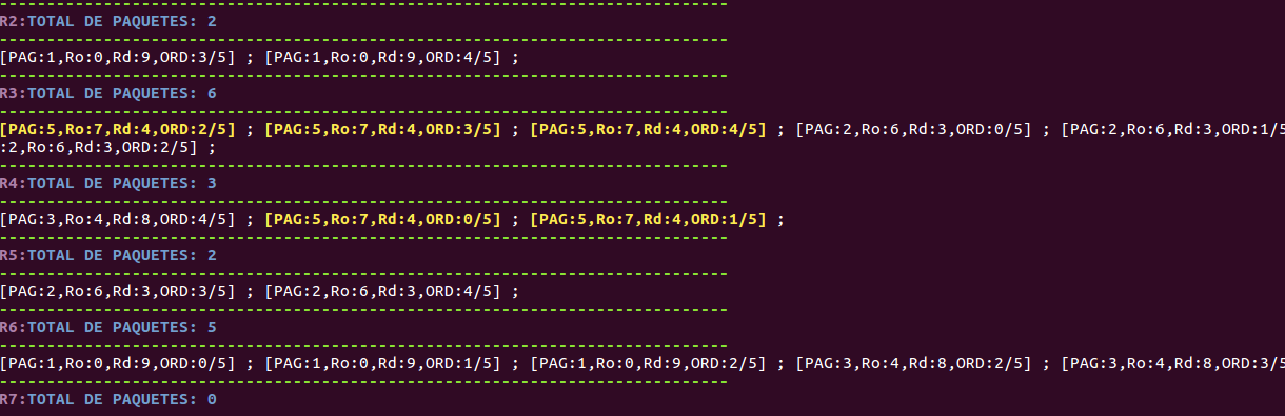
\includegraphics[width=\linewidth]{config_1_run5}}
\label{fig:config_1_run5}
\end{figure}

\begin{figure}[H] % Example image
\center{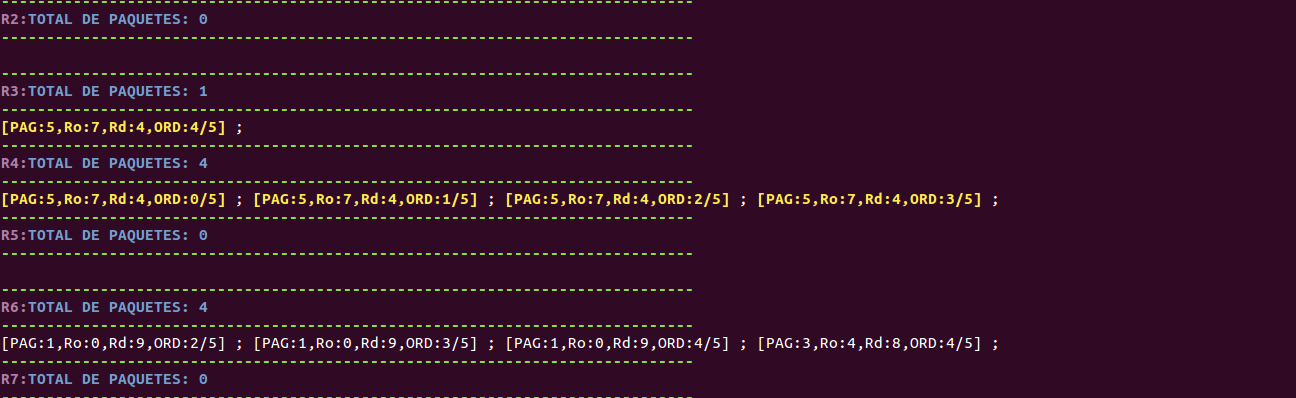
\includegraphics[width=\linewidth]{config_1_run6}}
\label{fig:config_1_run6}
\end{figure}

A consecuencia del ancho de banda de las Conexiones involucradas en la trayectoria y la demanda de paquetes, en 5to pasos de simulación se logra completar la página 5.

\begin{figure}[H] % Example image
\center{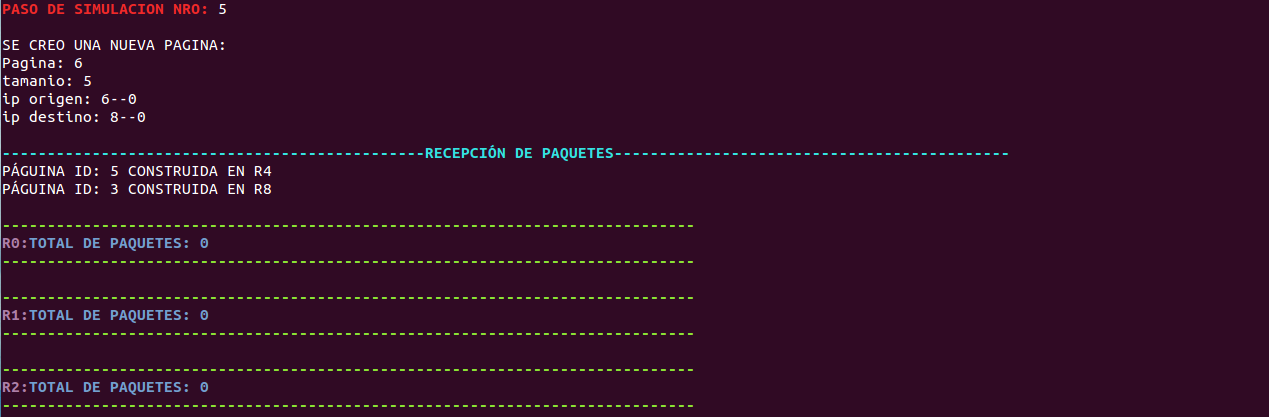
\includegraphics[width=\linewidth]{config_1_run7}}
\label{fig:config_1_run7}
\end{figure}

%----------------------------------------------------------------------------------------
%	CONCLUSION
%----------------------------------------------------------------------------------------

\section{Conclusion} % Major section
Finalizado el desarrollo del trabajo, de la ejecución del algoritmo de dijkstra pudimos apreciar que es una herramienta de gran utilidad y eficiencia.
Aplicamos la propiedad de popularización, junto con un controlador de versiones, la tarea de programación fue más ligera, con el diseño previamente establecido.
Además Pudimos dimensionar la potencialidad de las estructuras utilizadas: Nodo, Lista, Cola, Grafo. Inclusive, fue empleamos la estructura Cola, de manera iterativa, con el fin de conseguir igualdad al momento de selección de paquetes para enviar.
%%\lipsum[12-13]

%----------------------------------------------------------------------------------------
%	BIBLIOGRAPHY
%----------------------------------------------------------------------------------------

\begin{thebibliography}{99} % Bibliography - this is intentionally simple in this template

\bibitem[1]{Figueredo:2009dg}
 \textsc{Cormen, T.~C ; Leiserson, C.E~ ; Rivest, R.L~ } and \textsc{Stein, C~}
\textit{Introduction to Algorithms}, Third Edition
The MIT Press. Cambridge, Massachusetts	London, England, 2009
\newblock {\em Single-Source Shortest Paths}, 24:658--662.

\bibitem[2]{cplusplus.com}
http://www.cplusplus.com/forum/articles/10627/
\textit{Headers and Includes: Why and How} 2009

\bibitem[1]{choorucode.com}
http://choorucode.com/2010/07/22/c-fixing-cyclic-dependencies/
\textit{C++: Fixing Cyclic Dependencies} 2010

\end{thebibliography}

%----------------------------------------------------------------------------------------

\end{document}
